 \let\negmedspace\undefined
\let\negthickspace\undefined
\documentclass[journal]{IEEEtran}
\usepackage[a5paper, margin=10mm, onecolumn]{geometry}
\usepackage{lmodern} % Ensure lmodern is loaded for pdflatex
\usepackage{tfrupee} % Include tfrupee package

\setlength{\headheight}{1cm} % Set the height of the header box
\setlength{\headsep}{0mm}     % Set the distance between the header box and the top of the text

\usepackage{gvv-book}
\usepackage{gvv}
\usepackage{cite}
\usepackage{amsmath,amssymb,amsfonts,amsthm}
\usepackage{algorithmic}
\usepackage{graphicx}
\usepackage{textcomp}
\usepackage{xcolor}
\usepackage{txfonts}
\usepackage{listings}
\usepackage{enumitem}
\usepackage{mathtools}
\usepackage{gensymb}
\usepackage{comment}
\usepackage[breaklinks=true]{hyperref}
\usepackage{tkz-euclide} 
\usepackage{listings}                                      
\def\inputGnumericTable{}                                 
\usepackage[latin1]{inputenc}                                
\usepackage{color}                                            
\usepackage{array}                                            
\usepackage{longtable}
\usepackage{multicol}
\usepackage{calc}                                             
\usepackage{multirow}                                         
\usepackage{hhline}                                           
\usepackage{ifthen}                                           
\usepackage{lscape}
\begin{document}

\bibliographystyle{IEEEtran}
\vspace{3cm}

\title{9.7.12}
\author{EE24BTECH11052 - Rongali Charan}
% \maketitle
% \newpage
% \bigskip
{\let\newpage\relax\maketitle}

\renewcommand{\thefigure}{\theenumi}
\renewcommand{\thetable}{\theenumi}
\setlength{\intextsep}{10pt} % Space between text and floats


\numberwithin{equation}{enumi}
\numberwithin{figure}{enumi}
\renewcommand{\thetable}{\theenumi}
\textbf{Question:}
Solve the differential equation 
$\sbrak{\frac{e^{-2\sqrt{x}}}{\sqrt{x}} - \frac{y}{\sqrt{x}}}\frac{dx}{dy} = 1 \quad (x \neq 0)$
\begin{enumerate}
    \item \textbf{Theoretical Solution:}\\
   Rearranging the equation to standard form:
	\begin{align}
		\frac{dy}{dx} &= \frac{e^{-2\sqrt{x}} - y}{\sqrt{x}}\\
        \frac{dy}{dx} + \frac{y}{\sqrt{x}} &= \frac{e^{-2\sqrt{x}}}{\sqrt{x}}\\
        \text{This is in the form: } \frac{dy}{dx} + P(x)y &= Q(x)\\
        \text{where } P(x) = \frac{1}{\sqrt{x}} \text{ and } Q(x) &= \frac{e^{-2\sqrt{x}}}{\sqrt{x}}
    \end{align}
    The integrating factor is:
    \begin{align}
        \mu(x) &= e^{\int P(x)dx} = e^{\int \frac{dx}{\sqrt{x}}}\\
        &= e^{2\sqrt{x}}
    \end{align}
    Multiplying both sides by $\mu(x)$:
    \begin{align}
        e^{2\sqrt{x}}\frac{dy}{dx} + \frac{e^{2\sqrt{x}}}{\sqrt{x}}y &= \frac{e^{2\sqrt{x}}e^{-2\sqrt{x}}}{\sqrt{x}}\\
        \frac{d}{dx}(e^{2\sqrt{x}}y) &= \frac{1}{\sqrt{x}}\\
        e^{2\sqrt{x}}y &= 2\sqrt{x} + C\\
    x_0 = 1, y_0 = 0 \implies C=-2 \\   
   \therefore y = e^{-2\sqrt{x}}(2\sqrt{x} - 2)
    \end{align}   
    \item \textbf{Using method of finite differences:}\\
    The Method of Finite Differences approximates the solution using discrete steps.\\
    We know that:
    \begin{align}
        \frac{dy}{dx} &= \frac{e^{-2\sqrt{x}}-y}{\sqrt{x}}\\
        \lim_{h\to 0}\frac{y_{n+1}-y_n}{h} &= \frac{e^{-2\sqrt{x_n}}-y_n}{\sqrt{x_n}}\\
	    \approx \frac{y_{n+1}-y_n}{h}&=\frac{e^{-2\sqrt{x_n}}-y_n}{\sqrt{x_n}}\\
        \therefore y_{n+1} &= y_n + h\cdot\frac{e^{-2\sqrt{x_n}}-y_n}{\sqrt{x_n}}
    \end{align}
    
    The following steps were used:
    \begin{enumerate}
        \item Initialize $x_0=1$ and $y_0=0$
        \item Choose step size $h=0.01$ and number of steps $n=1000$ to ensure accuracy
        \item Generate points iteratively using:
        \begin{align}
            x_{n+1} &= x_n + h\\
            y_{n+1} &= y_n + h\cdot\frac{e^{-2\sqrt{x_n}}-y_n}{\sqrt{x_n}}
        \end{align}
    \end{enumerate}
    
The below graph shows the comparison between the curve that is obtained theoretically and the simulation curve(numerically generated points through iterations).
\end{enumerate}
\begin{figure}[htbp]
  \centering
  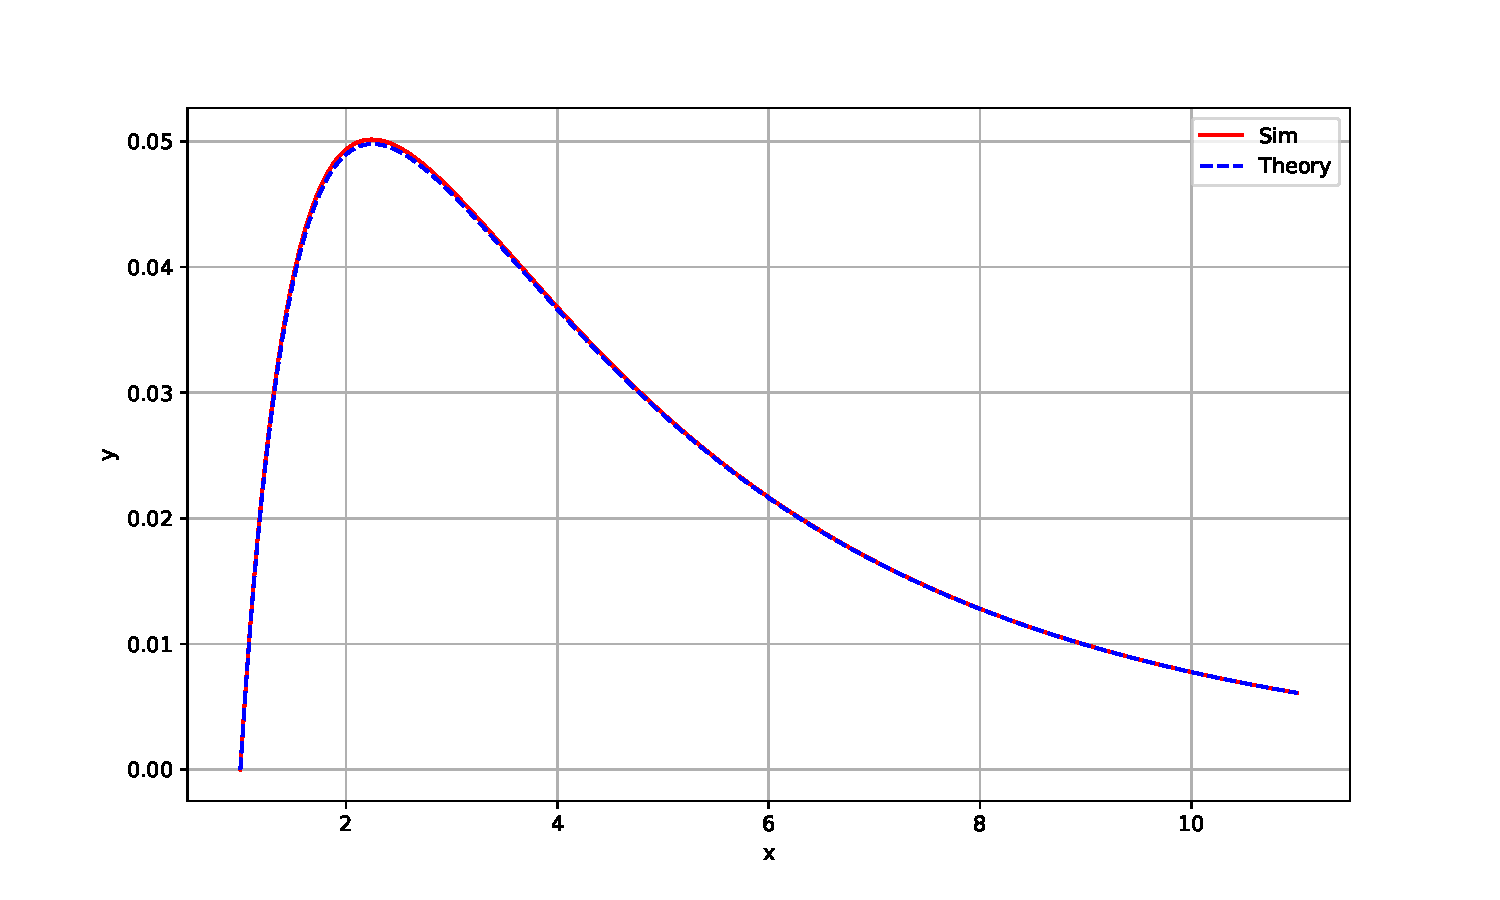
\includegraphics[width=\columnwidth]{figs/curve.pdf}
\end{figure}
\end{document}
